\section{Results}
\label{sec:Evaluation}
We collected data from $9$ subjects, each using our instrumented visualization for approximately $50$ minutes on a series of structured and unstructured tasks. We used the collected data to test the validity and effectiveness of collecting eye-tracking data in visualization space in two ways. 

First, we compared the similarity of our algorithm output to human annotation data, with the similarity between human annotations. We found that our results were on average as similar to human annotations as human annotations were similar to each other. Moreover, we conducted this analysis for all three viewed detection algorithms described in Sections~\ref{sec:AOIBasedViewedObjectDetection} to~\ref{sec:MehthodsIntelligentAlgorithm} and showed that the AOI based method (Section~\ref{sec:AOIBasedViewedObjectDetection}) performs poorly compared to the other two, and that the prediction component (Section~\ref{sec:MehthodsIntelligentAlgorithm}) improves detection accuracy by about $4\%$  (Figure~\ref{fig:quantitative}). 

Second, we demonstrate that our instrumentation method can provide relevant information by showing that viewed objects detected by our instrumentation align with the tasks we asked people to do. Moreover, we show that data collected in this was can be useful in analyzing visual behavior for data visualization users.  
We discuss the validity and benefits of these evaluation choices are discussed in Section~\ref{sec:Discussion}.

\subsection{Study Design }
\label{sec:EvalStudyDesign}

\textbf{Setup: } We used the visualization and data described in Section~\ref{sec:Methods}, and a lightweight $60$Hz EyeX eye-tracker from Tobii connected to a 17'' monitor. Subjects were seated approximately $30''$ away from the display. 

\textbf{Subjects:} We collected data from $9$ graduate and undergraduate students with ages ranging between $20$ years and $30$ years. Six of them were male and three were female. Subjects were paid $10$ for their participation. 

\textbf{Protocol:} Subjects were first given a description of the study's purpose and protocol. They were then introduced to our IMDB PivotPaths visualization and asked to perform a few training tasks to help them get accustomed with the visualization. This introductory part lasted on average $10$ minutes. The main section of the study followed, involved multiple instances of four types of tasks, and lasted approximately $50$ minutes. 


\textbf{Tasks:} We asked subjects to complete four types of tasks. We aimed to balance structured tasks and unstructured tasks. To solve the structured tasks, subjects had to consider a set of objects that was better defined and less variable than in unstructured tasks. This made it easier for us to test the degree to which our detection of viewed objects is aligned with the data required to complete the tasks. On the other hand, data collected for unstructured tasks may be better at informing designs of future analysis systems of such data. We limited the time we allowed subjects to spend on each task. This was done for two reasons: to limit the total duration of the study, and to make results comparable across time and users.

\begin{itemize}
\item \textbf{Task1 (structured):} Finding four commonalities between pairs of movies. The tasks were limited at three minutes each, and subjects solved the following four instances of this task: (i) Goodfellas and Raging bull (ii) Raiders of the Lost Ark and Indiana Jones and the Last Crusade; (iii) Invictus and Million Dollar Baby (iv) Inception and The Dark Knight Rises.  
\item \textbf{Task2 (structured):} Ranking collaborations between a director and three actors ($2$ minutes).  Subjects complete the following four task instances: Ang Lee, Tim Burton, James Cameron and David Fincher; 
\item \textbf{Task4 (semi-structured):} Given three movies, subjects were asked to recommend a fourth ($5$ minutes). Subjects solved three such tasks: 
\item \textbf{Task5 (unstructured):} Given a brief and incomplete description of the ``Brat Pack'', a group of young actors popular in the 80's, subjects were asked to find additional members and movies they acted in. Subjects solved one such task, in approximately $5$ minutes. 
\end{itemize}

\subsection{Results}
\subsubsection{Data collected automatically is similar to that of human annotators}
\label{sec:EvalResults}

We compared lists of viewed objects produced by our instrumentation to similar lists created by human coders. To this end, we enlisted the help of five coders and asked them to annotate data corresponding to one task of approximately three minutes, for each of six subjects.  Each coder spent approximately one hour on each subject. Four coders completed all assigned tasks, while one was able to finish only three of the six data sets. The six subjects were selected randomly and were the same for all five coders. We found that similarities between the results of human coders and the `intelligent' instrumentation described in Section~\ref{sec:MehthodsIntelligentAlgorithm} are very close to the similarities between the results of human coders. These results are shown in Figure~\ref{fig:quantitative} ( `intelligent' and `coder' columns).

Coders were asked to indicate what they thought the subjects looked at, and note the start and end time of each object's viewing, at a resolution of $100$ms. They were allowed to indicate multiple objects if they were unsure which of those objects was viewed. Coders used an application that allowed them to look at screen captures of the users' activity with overlaid gaze coordinates. 

We transformed the data provided by each coder for each user into a long vector with a position for each $100$ms that was analyzed, and their coding result for that particular $100$ms interval. We then created a similar representation from our automatically collected data. We defined a similarity measure between two such vectors as the percentage of temporally aligned cells from the two vectors that are equal. Equality between cells was defined as a non-empty intersection between their contents. Finally, we computed such similarities between each coder and the automatically generated annotation for each of the six subjects ($4$ coders $\times$ $6$ subjects $+$ $1$ coder $\times$ $3$ subject $=$ $27$ similarities), and similarities between all pairs of coders for each subject ( $3$ subjects $\times$ $4$ coders $+$ $4$ subjects $\times$ $5$ coders $=$ $48$ similarities). 

Moreover, the data we collected allowed us to do this analysis for all three approaches described in Section~\ref{sec:MethodsAlgorithmsViewedObjectDetection}. Specifically, if we only consider gaze scores $gs$ (Section~\ref{sec:AOIBasedViewedObjectDetection}) equal to one, we essentially have the output of the AOI based approach. If we limit the analysis to $gs$ scores alone, without the prediction component described in Section~\ref{sec:MehthodsIntelligentAlgorithm}, we have the output of the probabilistic approach described in Section~\ref{sec:ProbabilisticObjectDetection}. A comparison of how similar the output of each of these three approaches is to human annotation data is shown in Figure~\ref{fig:quantitative}, and demonstrates that the `intelligent' detection algorithm outperforms both other approaches.

\begin{figure}[htb]
  \centering
  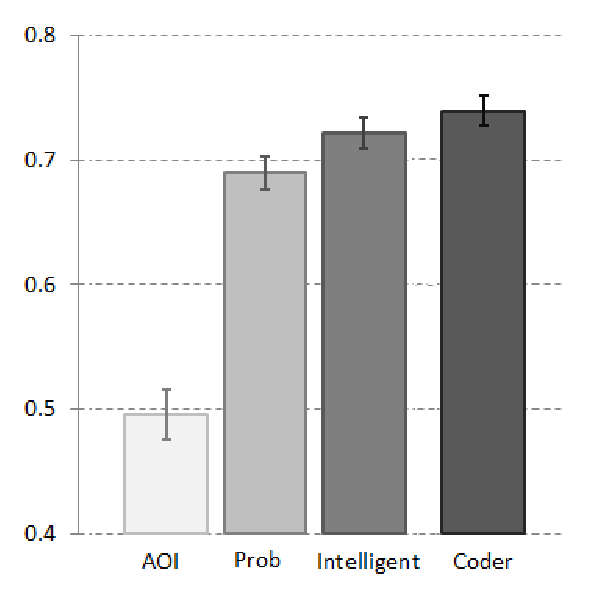
\includegraphics[width=0.6\linewidth]{images/algosComparison.eps}
  \caption{Comparison of different algorithms for analyzing eye tracking data.}
	\label{fig:quantitative}
\end{figure}


\subsubsection{Data collected automatically is relevant and useful}
\label{sec:EvalDataCollected}
We use two visual representations and analyses and show that data collected automatically using our approach are tightly correlated with the tasks that users had to do. Moreover, we show that such analyses can yield insights into how users perform tasks in an instrumented visualization. We chose this valuation method because it essentially provides evidence that the automatic instrumentation approach can be used to solve the inverse problem: an observer or analyst who is unfamiliar to a subject's intentions can determine what these are by looking at the subject's visual interest in particular data. 

\textbf{First}, we created heatmap representations from our collected data (Figure~\ref{fig:heatmap}). We listed viewed objects vertically and discretized viewing scores, using averaging, into $500ms$ intervals, which we arranged horizontally. Thus, time is shown horizontally, viewed objects vertically, and intensity of heatmap cells indicate the degree to which an object was viewed at a given moment in time. The viewed objects listed vertically were colored based on their type (movie, actor, director, genre) and could be sorted by either first time they were viewed, amount of viewing activity, or type. 

Figure~\ref{fig:heatmap}, left, shows the results for a subject performing the second instance of task 1: finding commonalities between two Indiana Jones movies (see Section~\ref{sec:EvalStudyDesign}). The heatmap is ordered by the amount of visual attention that the subject dedicated to each element in the visualization. We notice that elements at the top of the heatmap are tightly connected to the subject's  task.   

Figure~\ref{fig:heatmap}, right, shows a subject's results for one of the instances of task 3, which was significantly less structured than task 1 (see Section~\ref{sec:EvalStudyDesign}). This heatmap  was sorted by the first time each object was viewed and shows how subjects were moving through different aspects of the analyses, and revisiting them at different moments in time. 

\begin{figure*}[!ht]
  \centering
  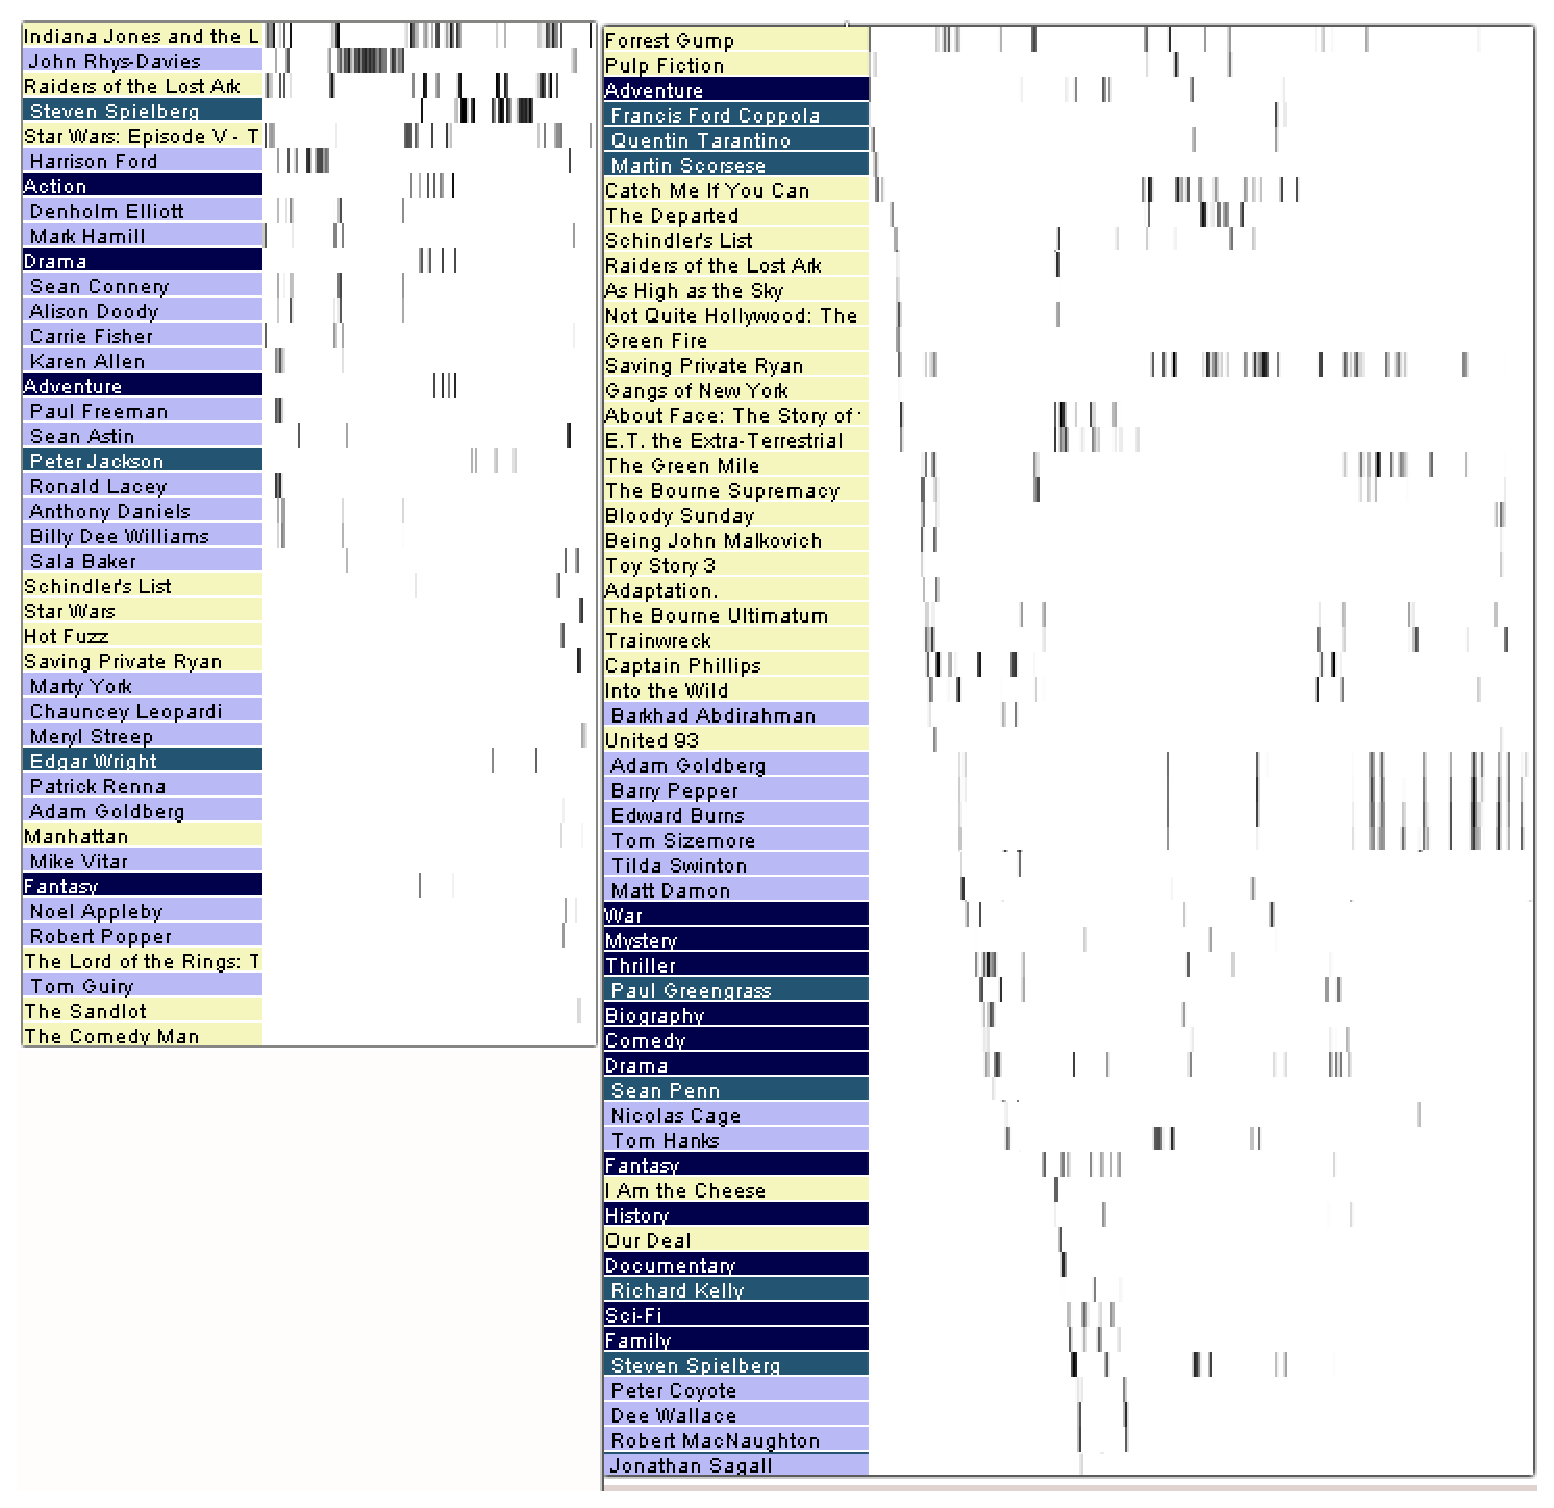
\includegraphics[width=0.75\linewidth]{images/heatmaps.eps}
  \caption{Heatmap views of one subject's activity on two tasks; time, in 500ms increments, are shown horizontally; viewed objects are viewed vertically; cell darkness indicates viewing intensity (black: high; white: low). (Top left) Data for the task 1.ii (see Section~\ref{sec:EvalStudyDesign}); viewed items are ordered by decreasing total amount they were viewed. (Bottom left) Data for the task 1.ii (see Section~\ref{sec:EvalStudyDesign}); viewed items are ordered by category (genre, director, movie, actor). (Right) Data for the task 1.ii (see Section~\ref{sec:EvalStudyDesign} 4.1); viewed items are ordered by first time they were seen. 
}
	\label{fig:heatmap}
\end{figure*}


\textbf{Second}, we formalized the relevance of each visual item to a particular task and plot this relevance against the amount of interest that each item attracted, as shown in Figure~\ref{fig:RelevanceDiagram}. These plots illustrate the degree to which task relevance impacts the amount that each visual item is tended to by subjects, and aimed to demonstrate that our instrumentation captures relevant data.  

We formalize the relevance of a visual item to a task, as the network minimum distance between that item and any item mentioned in the task description.  This definition is not complete as items might be relevant to a task even though they are not directly mentioned in the description.  For instance, items that eventually constitute a subject's answer will elicit more of the subject's attention. Moreover, this definition is particular to the visualization we instrumented.

A few insights can be drawn from analyzing these images. First, even though many items were shown to subjects during their tasks, only a few were viewed for significant periods of time, and many were not viewed at all. In fact, the interest in a particular item drops exponentially with that item's relevance to the task, which aligns with knowledge that people's perception is goal-driven.  Second, the types of data that users view more are correlated to each task particularities. For example, task 3 involved movie recommendations and Figure~\ref{fig:RelevanceDiagram}(c) illustrates that genres and directors were viewed significantly more than in task 4, which involved determining the identify of a group of actors. 



\begin{figure}[!htb]
  \centering
  \includegraphics[width=0.9\linewidth]{images/RelevanceDiagramTask1.eps}
	\caption*{Relevance Diagram Task 1}
	\includegraphics[width=0.61\linewidth]{images/RelevanceDiagramTask2.eps}
	\caption*{Relevance Diagram Task 2}
	\includegraphics[width=0.71\linewidth]{images/RelevanceDiagramTask3.eps}
	\caption*{Relevance Diagram Task 3}
	\includegraphics[width=\linewidth]{images/RelevanceDiagramTask4.eps}
	\caption*{Relevance Diagram Task 4}
  \captionof{figure}{Relevance Diagram Task 1}
	\label{fig:RelevanceDiagram}
\end{figure}





\subsubsection{Assumptions about viewing transition patterns hold}
We analyzed common viewing-transition patterns in the data we collected. Examples include how often our subjects change views from a genre to an un-highlighted item versus to a highlighted one, or how often subjects transition between connected items and unconnected items. We found that the assumptions described in Section~\ref{sec:Methods}, that users show a preference to transition their view to connected or highlighted items, holds. The data is summarized in the last columns  (adjusted transitions) of the panels in Table~\ref{tab:TransitionFromMovie}.

To this end, we first discarded the prediction component from our collected data, since the prediction represents the assumption we try to test, and would thus bias the data. We counted viewing transitions between all types of objects to all other types of objects, and we separated transitions to connected objects and to highlighted objects from all other ones, as seen in the first columns in Table~\ref{tab:TransitionFromMovie}.  For example, after viewing a movie, a user could view either a director, or an actor, or a genre, each of which can be either connected or unconnected to the movie, and highlighted or not. A subject could also transition between two movies, and, since movies are not connected to each other in our visualization, the only options are to view a highlighted or un-highlighted movie.  We note that we skipped transitions to or from empty space.  

The transition counts between different types of objects are shown in the third columns of panels in Table~\ref{tab:TransitionFromMovie}, and their translation into probabilities, computed by normalizing transitions in each category by the total number of transitions, is listed in the fourth columns of Table~\ref{tab:TransitionFromMovie}. 

However, these numbers could be slightly misleading because they do not take into account the number of objects in each category (e.g., actor, movie, unconnected, connected, highlighted) that a  subject could potentially transition to at any given point in time. For example, when a subject transitions their gaze from a movie to an actor, there are typically many more unconnected and un-highlighted actors to choose from, than there are actors that are either connected to the current movie and/or highlighted. Assuming a movie is connected to two actors and there are another eight unconnected items in the view, if there was no transitioning preference for either connected or unconnected items, the probability to jump to a connected item would be $0.2$, and to jump to an unconnected item it would be $0.8$. If however, we observe that users jump to one of the two connected items in $50\%$ of cases, and to unconnected items also in $50\%$ of cases, then there is clearly a significant bias towards viewing connected items together.

To account for this, every time we counted a transition between two visual items, we also counted all options available to a user at that point, given the state and structure of the visualization. Then, we used these counts to adjust the probabilities computed in Table~\ref{tab:TransitionFromMovie}. For example, even though there were 793 transitions from a movie to an unconnected actor, and just 228 to a connected one, there were many more opportunities for a subject to jump to an unconnected item than to a connected one. The adjusted probabilities indicate that in fact a subject is almost five times more likely to choose to view a connected actor after they viewed a movie. A quick inspection of the contents of Table~\ref{tab:TransitionFromMovie} will show that the assumptions we made in Section~\ref{sec:Methods} hold. Moreover, this type of analysis can be useful in helping us understand how visualizations are used and how workflows are approached by users.

\begin{table}[htbp]	
	\centering
		\begin{tabular}{|c|c|c|c|c|}
			\hline
			 \multicolumn{2}{ |l| }{Movie to}  &\shortstack{	No. of  \\ Transitions} 	&\shortstack{transition \\ prob.}	&\shortstack{	adjusted \\ transition \\ prob.}\\ \hline
      \multirow{4}{*}{Actor}	&-	&793	&0.076	&0.004	\\	\cline{2-5}
															&H	&147	&0.014	&0.032	\\	\cline{2-5}
															&C	&228	&0.022	&0.019	\\	\cline{2-5}
															&CH	&616	&0.059	&0.089	\\	\hline
				\multirow{2}{*}{Movie}	&-	&5727	&0.548	&0.131	\\	\cline{2-5}
																&H	&1798	&0.172	&0.368	\\	\hline
				\multirow{4}{*}{Director}	&-	&304	&0.029	&0.01	\\	\cline{2-5}
																	&H	&37	&0.004	&0.051	\\	\cline{2-5}
																	&C	&51	&0.005	&0.027	\\	\cline{2-5}
																	&CH	&174	&0.017	&0.135	\\	\hline
				\multirow{4}{*}{Genre}	&-	&193	&0.018	&0.005	\\	\cline{2-5}
																&H	&40	&0.004	&0.027	\\	\cline{2-5}
																&C	&69	&0.007	&0.015	\\	\cline{2-5}
																&CH	&282	&0.027	&0.087	\\	\hline
					\multicolumn{2}{ |l| }{Total}	&10459	&1	&1	\\		
				\hline
		\end{tabular}		
		\caption*{(a)Transitions from Movies}\smallskip
		
		\begin{tabular}{|c|c|c|c|c|}
			\hline
			 \multicolumn{2}{ |l| }{Actor to}  &\shortstack{	No. of  \\ Transitions} 	&\shortstack{transition \\ prob.}	&\shortstack{	adjusted \\ transition \\ prob.}\\ \hline
						 \multirow{2}{*}{Actor}	&-	&4711	&0.533	&0.032	\\	\cline{2-5}
																		&H	&2164	&0.245	&0.372	\\	\hline
							\multirow{4}{*}{Movie}	&-	&839	&0.095	&0.031	\\	\cline{2-5}
																			&H	&213	&0.024	&0.113	\\	\cline{2-5}
																			&C	&386	&0.044	&0.157	\\	\cline{2-5}
																			&CH	&352	&0.04	&0.236	\\	\hline
							\multirow{2}{*}{Director}	&-	&68	&0.008	&0.003	\\	\cline{2-5}
																				&H	&29	&0.003	&0.034	\\	\hline
							\multirow{2}{*}{Genre}	&-	&43	&0.005	&0.002	\\	\cline{2-5}
																			&H	&39	&0.004	&0.02	\\	\hline
								\multicolumn{2}{ |l| }{Total}	&8844	&1	&1	\\	
	\hline

		\end{tabular}
	\caption*{(b)Transitions from Actors}\smallskip
	\begin{tabular}{|c|c|c|c|c|}
			\hline
			 \multicolumn{2}{ |l| }{Director to}  &\shortstack{	No. of  \\ Transitions} 	&\shortstack{transition \\ prob.}	&\shortstack{	adjusted \\ transition \\ prob.}\\ \hline
       \multirow{2}{*}{Actor}	&-	&71	&0.042	&0.001	\\	\cline{2-5}
															&H	&24	&0.014	&0.011	\\	\hline
			\multirow{4}{*}{Movie}	&-	&271	&0.162	&0.031	\\	\cline{2-5}
														&H	&55	&0.033	&0.121	\\	\cline{2-5}
														&C	&130	&0.077	&0.108	\\	\cline{2-5}
														&CH	&93	&0.055	&0.139	\\	\hline
			\multirow{2}{*}{Director}	&-	&384	&0.229	&0.054	\\	\cline{2-5}
																&H	&160	&0.095	&0.299	\\	\hline
			\multirow{2}{*}{Genre}	&-	&256	&0.153	&0.026	\\	\cline{2-5}
															&H	&234	&0.139	&0.211	\\	\hline
				\multicolumn{2}{ |l| }{Total}	&1678	&1	&1	\\	
				\hline
		\end{tabular}
		\caption*{(c)Transitions from Director}\smallskip
		\begin{tabular}{|c|c|c|c|c|}
			\hline
			 \multicolumn{2}{ |l| }{Genre to}  &\shortstack{	No. of  \\ Transitions} 	&\shortstack{transition \\ prob.}	&\shortstack{	adjusted \\ transition \\ prob.}\\ \hline
       \multirow{2}{*}{Actor}	&-	&61	&0.03	&0	\\	\cline{2-5}
															&H	&32	&0.016	&0.011	\\	\hline
				\multirow{4}{*}{Movie}	&-	&229	&0.113	&0.012	\\	\cline{2-5}
																&H	&46	&0.023	&0.077	\\	\cline{2-5}
																&C	&172	&0.085	&0.024	\\	\cline{2-5}
																&CH	&138	&0.068	&0.135	\\	\hline
				\multirow{2}{*}{Director}	&-	&282	&0.139	&0.015	\\	\cline{2-5}
																	&H	&195	&0.096	&0.383	\\	\hline
				\multirow{2}{*}{Genre}	&-	&348	&0.172	&0.013	\\	\cline{2-5}
																&H	&526	&0.259	&0.328	\\	\hline
					\multicolumn{2}{ |l| }{Total}	&2029	&1	&1	\\	
			\hline
		\end{tabular}
		\caption*{(d)Transitions from Genres}\smallskip
	\captionof{table}{Transitions among different elements.}
	\label{tab:TransitionFromMovie}
\end{table}